\chapter{Einführung in Python und erste Schleifen}\label{ch:K02_Intro}


Um mit einem Computer zu \enquote{sprechen}, brauchen wir eine Sprache, die er versteht: Eine \textbf{Programmiersprache}\index{Programmiersprache}. Indem wir Programme schreiben, geben wir dem Computer klare Anweisungen, welche Aufgaben er erledigen soll. In diesem Skript nutzen wir die neueste Version der Programmiersprache \emph{Python}.

Genau wie unsere menschlichen Sprachen haben Programmiersprachen Wörter mit einer festen Bedeutung. Wörter, die dem Computer sagen, was er tun soll, nennen wir Befehlswörter oder einfach \textbf{Befehle}.

Ein \textbf{Programm} ist im Grunde eine Reihe von Befehlen in einer Programmiersprache, die zusammen eine bestimmte Aufgabe lösen. Stell dir ein Programm als eine genaue Anleitung vor, die ein Computer Schritt für Schritt abarbeiten kann.

Das Hauptziel des Programmierens ist die Automatisierung von Abläufen. Wir übertragen die Ausführung einer Aufgabe komplett an den Computer. Deshalb muss ein Programm absolut eindeutig sein und genau beschreiben, was zu tun ist. Es darf keine Missverständnisse geben.

In diesem Kapitel schreiben Sie Ihre ersten eigenen Programme. Dabei lernen Sie das Konzept der Schleifen kennen. Schleifen sind unglaublich praktisch, denn sie ermöglichen es, wiederkehrende Aufgaben automatisch mehrfach auszuführen. Sie werden sehen, wie nützlich das in vielen Alltagssituationen ist!

\section{Einige grundlegende Befehle und Operationen}

\subsection{\texorpdfstring{\lstinline|print|}{print}-Funktion und built-in Funktionen}
In unserem \texttt{Hello, World!}-Programm (\cref{listing:hello_world}) haben wir bereits die Python-Funktion \lstinline|print(...)|\index{print} gesehen.
Diese Funktion ermöglicht es uns, Dinge (genauer: Python-Objekte) auszugeben (\enquote{zu printen}) und dadurch für den User im Terminal sichtbar zu machen. Die \lstinline|print|-Funktion ist eine \emph{built-in Funktion}\index{built-in Funktion}, das heisst, sie ist direkter Bestandteil der Python-Sprache und ist in Python standardmässig verfügbar.

\begin{myexample}\label{myexample:prints}
Weitere Beispiele von Prints in Python:
\lstinputlisting[language=Python,caption=\texttt{prints.py},label=listing:prints]{Grundlagen_Info/00_Programmieren/Skript/Code/K02_Intro/prints.py}
\end{myexample}

\begin{myremark}\label{myremark:builtin}
	Unter dem Link
	\begin{center}
		\url{https://docs.python.org/3/library/functions.html#print}
	\end{center}
	finden Sie eine Übersicht aller built-in Funktionen in Python. Wir empfehlen Ihnen für diesen Link ein Lesezeichen (Bookmark) in Ihrem Webbrowser zu erstellen.
	Einige dieser Funktionen werden wir im Folgenden gemeinsam kennenlernen.
\end{myremark}

\subsection{Python-Kommentare}
Kommentare\index{Kommentar} in Python dienen dazu, Programmcode genauer zu beschreiben. Kommentare werden von Python vollständig ignoriert und dienen lediglich dem besseren Verständnis des (menschlichen) Lesers.
\begin{myexample}\label{myexample:kommentare}
Dieses Beispiel zeigt die Funktionsweise von Zeilenkommentaren und Blockkommentaren.
\lstinputlisting[language=Python,caption=\texttt{kommentare.py},label=listing:kommentare]{Grundlagen_Info/00_Programmieren/Skript/Code/K02_Intro/kommentare.py}
\end{myexample}

\subsection{Einfache Arithmetik}
In Python lassen sich einfache Rechenoperationen ähnlich wie bei einem Taschenrechner angeben. Dabei hält sich Python an die gewohnten Konventionen wie zum Beispiel \enquote{Punkt vor Strich}. Symbole gängiger arithmetischer Operationen sind in \cref{tab:arithm-op} zusammengefasst.

\begin{myoverview}[arithmetische Operationen in Python]
	\begin{table}[H]
		\centering
		\begin{tabular}{c|c}
			\textbf{mathematische Operation} & \textbf{In Python} \\\midrule\midrule
			Addition                         & \lstinline|+|      \\\midrule
			Subtraktion                      & \lstinline|-|      \\\midrule
			Multiplikation                   & \lstinline|*|      \\\midrule
			Division                         & \lstinline|/|      \\\midrule
			Potenzieren                      & \lstinline|**|
		\end{tabular}
		\caption{arithmetische Operationen in Python}
		\label{tab:arithm-op}
	\end{table}
\end{myoverview}
\begin{myexample}\label{myexample:basisoperationen}
Wir haben einige typische Rechenoperationen für Sie aufgeführt:
\lstinputlisting[language=Python,caption=\texttt{basisoperationen.py},label=listing:basisoperationen]{Grundlagen_Info/00_Programmieren/Skript/Code/K02_Intro/basisoperationen.py}
\end{myexample}

\section{Erste Zeichnungen mit der Python-Turtle}
Für den Einstieg in das Programmieren ist es didaktisch sinnvoll, mit der Python-Turtle zu starten. Genau dies werden wir hier tun! Wir werden der Turtle Instruktionen erteilen, damit sie für uns bestimmte Bilder und geometrische Formen zeichnet. Der didaktische Vorteil des Arbeitens mit der Turtle liegt in dem grafischen Output. Dieser lässt Sie (meist) sofort selber erkennen, was Ihr Programm macht und auch potenzielle Fehler lassen sich in der Regel recht einfach auffinden.

Um mit der Turtle arbeiten zu können, müssen Sie das \lstinline|turtle|-Modul durch den Befehl \lstinline|import turtle| zu Beginn des Programms (ganz oben) importieren. Ein Modul ist eine \enquote{Erweiterung} von Python, so dass wir zusätzlich zu den \emph{built-in functions} auch die Befehle des Moduls verwenden können.

Mit dem Ausdruck \lstinline|import turtle as t| sagen wir, dass wir das Modul \lstinline|turtle| in unser Programm importieren und dieses Modul innerhalb des Programms mit dem Ausdruck \lstinline|t| benennen werden (wird könnten auch \lstinline|import turtle as bliblablup| schreiben, dies wäre jedoch wohl weniger praktisch.

\cref{listing:strich} lässt die Turtle einen Strich mit einer Länge von $140$ zeichnen. \cref{listing:dreieck} zeichnet ein gleichseitiges Dreieck mit Seitenlänge $100$.

\lstinputlisting[language=Python,caption=\texttt{strich.py},label=listing:strich]{Grundlagen_Info/00_Programmieren/Skript/Code/K02_Intro/strich.py}
\lstinputlisting[language=Python,caption=\texttt{dreieck.py},label=listing:dreieck]{Grundlagen_Info/00_Programmieren/Skript/Code/K02_Intro/dreieck.py}

\begin{myremark}\label{myremak:turtledok}
	Unter dem Link
	\begin{center}
		\url{https://docs.python.org/3/library/turtle.html#module-turtle}
	\end{center}
	finden Sie eine Übersicht aller Turtle-Funktionen. Wir empfehlen Ihnen für diesen Link ein Lesezeichen (Bookmark) in Ihrem Webbrowser zu erstellen.
	Einige dieser Funktionen werden wir im Folgenden gemeinsam kennenlernen.
\end{myremark}

\begin{myexercise}\label{myexercise:Haus}
	Vervollständigen Sie die gegebene Vorlage, um ein Haus ähnlich dem in \cref{fig:Haus} mithilfe der Turtle zu zeichnen.
	\begin{figure}[H]
		\centering
		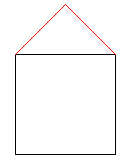
\includegraphics[width=0.3\textwidth]{Grundlagen_Info/00_Programmieren/Skript/Figures/Haus.png}
		\caption{Traumhaus}
		\label{fig:Haus}
	\end{figure}
	\begin{itemize}
		\item Die Längen dürfen Sie selber bestimmen.
		\item Das Schrägdach soll in roter Farbe gezeichnet werden und muss ein gleichschenkliges und rechtwinkliges Dreieck sein.
		\item Das Programm soll die Länge der Kathete dieses rechtwinkligen Dreieckes mit einem Print ausgeben.
	\end{itemize}
	\lstinputlisting[language=Python,caption=\texttt{haus\_vorlage.py},label=listing:haus_vorlage]{Grundlagen_Info/00_Programmieren/Skript/Code/K02_Intro/haus_vorlage.py}
	\begin{myanswer}
		\lstinputlisting[language=Python,caption=\texttt{haus.py},label=listing:haus]{Grundlagen_Info/00_Programmieren/Skript/Code/K02_Intro/haus.py}
	\end{myanswer}
\end{myexercise}


\begin{myexercise}\label{myexercise:dreizack}
	Schreiben Sie ein Programm um einen Dreizack möglichst ähnlich dem in \cref{fig:Dreizack} mithilfe der Turtle zu zeichnen.
	\begin{figure}[H]
		\centering
		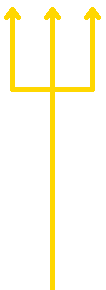
\includegraphics[width=0.2\textwidth]{Grundlagen_Info/00_Programmieren/Skript/Figures/dreizack.png}
		\caption{Poseidons Dreizack}
		\label{fig:Dreizack}
	\end{figure}
	Tipp: Durchsuchen Sie die Turtle-Dokumentation (siehe \cref{myremak:turtledok}) um zu lernen, wie die Stiftbreite und Stiftfarbe  (hier: \verb|"gold"|) angepasst werden kann.
	\begin{myanswer}
		Diese Musterlösung finden Sie in \cref{sec:K02_sol}.
	\end{myanswer}
\end{myexercise}

\section{Schleifen}
Schleifen\index{Schleife} (Englisch: \emph{loops}\index{loop}) ermöglichen uns, Prozesse zu wiederholen.

\begin{myexample}\label{myexample:Treppe}
In \cref{fig:Treppe} ist eine Treppe gezeigt. Wie können wir diese Treppe mithilfe der Turtle zeichnen? Mit unserem bisherigen Wissen wäre dies sehr mühsam:
\lstinputlisting[language=Python, numbers=left]{Grundlagen_Info/00_Programmieren/Skript/Code/K02_Intro/treppe_naiv.py}

\begin{figure}[H]
	\centering
	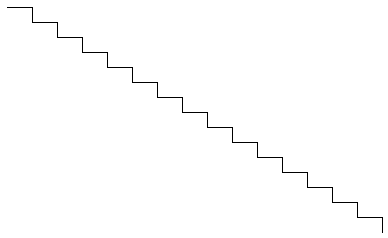
\includegraphics[width=0.5\textwidth]{Grundlagen_Info/00_Programmieren/Skript/Figures/treppe.png}
	\caption{Stairway to Heaven}
	\label{fig:Treppe}
\end{figure}
Stellen Sie sich vor, Sie müssten eine Treppe mit $10000$ Stufen zeichnen \emoji{face-with-monocle}.
\end{myexample}

\cref{myexample:Treppe} zeigt auf, dass wir eine praktikable Methode zum häufigen Wiederholen von Mustern oder Prozessen benötigen. In Python lassen sich Wiederholungen mit Schleifen realisieren.
Die Treppe aus \cref{myexample:Treppe} lässt sich mit einer sogenannten \lstinline|for|-Schleife ganz einfach wie in \cref{listing:treppe} realisieren.
\lstinputlisting[language=Python,numbers=left,caption=\texttt{treppe.py},label=listing:treppe]{Grundlagen_Info/00_Programmieren/Skript/Code/K02_Intro/treppe.py}

Dabei wird folgender Ausdruck:
\begin{center}
	\lstinline|for _ in range(15):|
\end{center}
der \emph{Schleifenkopf}\index{Schleife!Kopf einer} der Schleife genannt. Die vier Zeilen (6 -- 9) werden \emph{Schleifenkörper}\index{Schleife!Körper einer} der Schleife genannt, wie im unten stehenden Code zu sehen ist.

\begin{figure}[H] % not really a figure, just acts as non-floating container
	\centering
	\begin{lstlisting}[escapechar=!]
for _ in range(15):!\tikzmark{code2}\tikzmark{repeatStart}!              !\tikzmark{comment2}!
    t.fd(15)!\tikzmark{bodyStart}!                               
    t.lt(90)
    t.fd(25)
    t.rt(90)!\tikzmark{bodyEnd}!       !\tikzmark{repeatEnd}!
\end{lstlisting}
	\begin{tikzpicture}[overlay, remember picture,
			every node/.style={draw=red!50,fill=red!50!white,text=black,rounded corners}]
		\drawArrow{code2}{comment2}{\footnotesize Schleifenkopf}{red!50!white}
		\drawBrace{1em}{repeatStart}{repeatEnd}{\footnotesize Schleife}{.45}{}{}
		\drawBrace{0em}{bodyStart}{bodyEnd}{\footnotesize\emph{Körper} der Schleife}{.8}{}{8.5em}
	\end{tikzpicture}
\end{figure}

Der Schleifenkörper ist (in Python) daran erkennbar, dass er (relativ zu dem Schleifenkopf) nach rechts eingerückt (Englisch: \emph{indented}) ist. Diese Einrückung erreichen wir in VS Code durch das einfache Drücken der Tabulator-Taste (\keys{\tab}). Wir können Code auch wieder um einen Tab nach links rücken, indem wir den entsprechenden Code zuerst selektieren (einfärben) und danach die Shift-Taste sowie die Tabulator-Taste gleichzeitig drücken (\keys{\shift + \tab}). In anderen Programmen als VS Code kann es sein, dass die Tastaturkombination dafür eine andere ist.

\begin{myexercise}\label{myexercise:zackenSchleife}
	Verwenden Sie eine Schleife, folgendes Bild zu zeichnen:
	\begin{figure}[H]
		\centering
		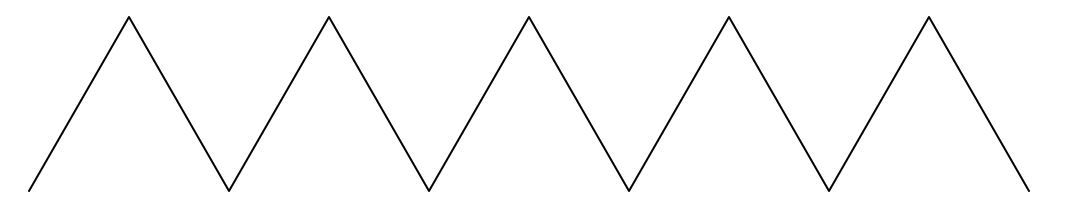
\includegraphics[width=0.6\textwidth]{Grundlagen_Info/00_Programmieren/Skript/Figures/ZackenSchleife.png}
		\caption{Zacken bestehend aus gleichseitigen Dreiecken}
		\label{fig:ZackenSchleife}
	\end{figure}
	\begin{myanswer}
		\lstinputlisting[language=Python,caption=\texttt{zacken\_schleife.py},label=listing:dreieckSchleife]{Grundlagen_Info/00_Programmieren/Skript/Code/K02_Intro/zacken_schleife.py}
	\end{myanswer}
\end{myexercise}

% Für eine vollständige Auflistung aller Shortcuts schauen Sie sich bitte \cref{sec:shortcuts} an.
\begin{myexercise}\label{myexercise:approximationKreis}
	In \cref{fig:ApproximationKreis} wird gezeigt, wie ein Kreis schrittweise durch regelmässige Polygone\footnote{\url{https://de.wikipedia.org/wiki/Regelm\%C3\%A4\%C3\%9Figes\_Polygon}} approximiert (angenähert)
	\begin{figure}[H]
		\centering
		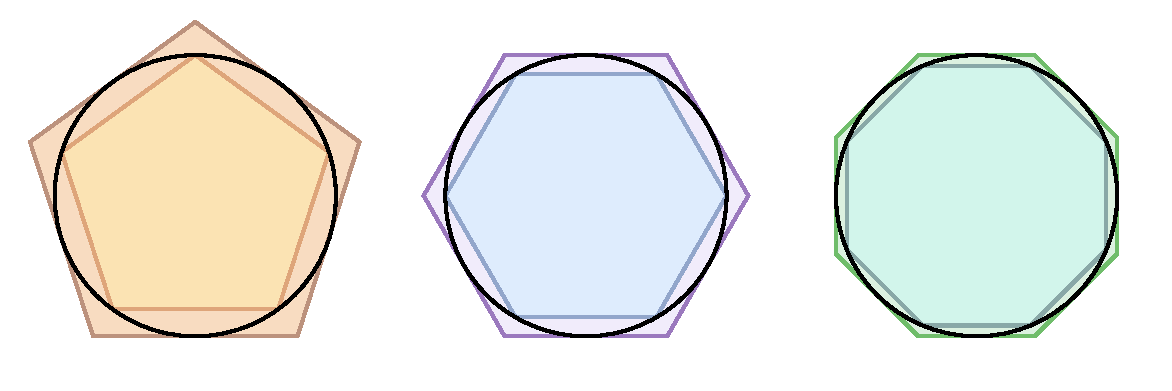
\includegraphics[width=0.5\textwidth]{Grundlagen_Info/00_Programmieren/Skript/Figures/approximation_kreis.pdf}
		\caption{Schrittweise Annäherung an einen Kreis durch ein- beziehungsweise umbeschriebene regelmässige Polygone (links: 5-Ecke, mittels: 6-Ecke, rechts: 8-Ecke).}
		\label{fig:ApproximationKreis}
	\end{figure}
	\begin{itemize}
		\item Lassen Sie die Turtle in demselben Bild ein regelmässiges 5-Eck, ein regelmässiges 6-Eck sowie ein regelmässiges 8-Eck zeichnen.
		\item Die Orientierungen und Grössen der Figuren spielen dabei keine Rolle.
		\item Die Figuren sollen sich nicht überschneiden.
		\item Sie wollen die Turtle bewegen, ohne dabei zu zeichen? Schauen Sie sich die Funktionen \lstinline|t.penup()| und \lstinline|t.pendown()| in der \href{https://docs.python.org/3/library/turtle.html}{turtle-Dokumentation} an (suchen Sie nach diesen Befehlen mit dem Shortcut \keys{\ctrl + F} (Windows) oder \keys{\cmd + F} (MacOS)).
	\end{itemize}
	\begin{myanswer}
		\lstinputlisting[language=Python,caption=\texttt{regelmaessige\_polygone.py},label=listing:regelmaessige_polygone]{Grundlagen_Info/00_Programmieren/Skript/Code/K02_Intro/regelmaessige_polygone.py}
	\end{myanswer}
\end{myexercise}

\subsection{geschachtelte Schleifen}
In der Praxis verwenden wir oft Schleifen innerhalb von Schleifen. Solche Schleifen nennt man \textbf{geschachtelte Schleifen}\index{Schleife!geschachtelte}.

\begin{myexample}\label{myexample:quadrate}
In diesem Beispiel zeichnen wir, mithilfe geschachtelter Schleifen, drei nebeneinander liegende Quadrate:
\lstinputlisting[language=Python,caption=\texttt{quadrate.py},label=listing:quadrate]{Grundlagen_Info/00_Programmieren/Skript/Code/K02_Intro/quadrate.py}
\end{myexample}

\begin{myexercise}\label{myexercise:reihenhaus}
	Zeichnen Sie ein Reihenhaus, bestehend aus fünf nebeneinander liegenden Häusern, die alle gleich aussehen (siehe \cref{fig:Reihenhaus}). Verwenden Sie den Code, den Sie in \cref{myexercise:Haus} erstellt haben, als Vorlage für die Form eines einzelnen Hauses.
	\begin{figure}[H]
		\centering
		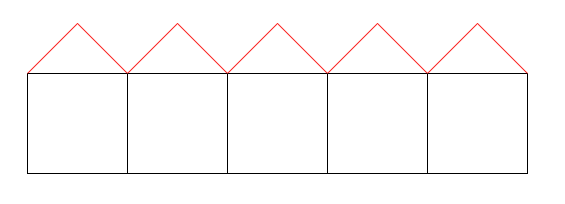
\includegraphics[width=0.5\textwidth]{Grundlagen_Info/00_Programmieren/Skript/Figures/Reihenhaus.png}
		\caption{Reihenhaus}
		\label{fig:Reihenhaus}
	\end{figure}
	\begin{myanswer}
	\lstinputlisting[language=Python,caption=\texttt{reihenhaus.py},label=listing:blume]{Grundlagen_Info/00_Programmieren/Skript/Code/K02_Intro/reihenhaus.py}
\end{myanswer}
\end{myexercise}

\begin{myexercise}\label{myexercise:Blume}
Zeichnen Sie die folgenden Blume mit der Turtle. Tipp: Es handelt sich dabei um $10$ Quadrate, die jeweils um $36$ Grad gedreht sind.
\begin{figure}[H]
	\centering
	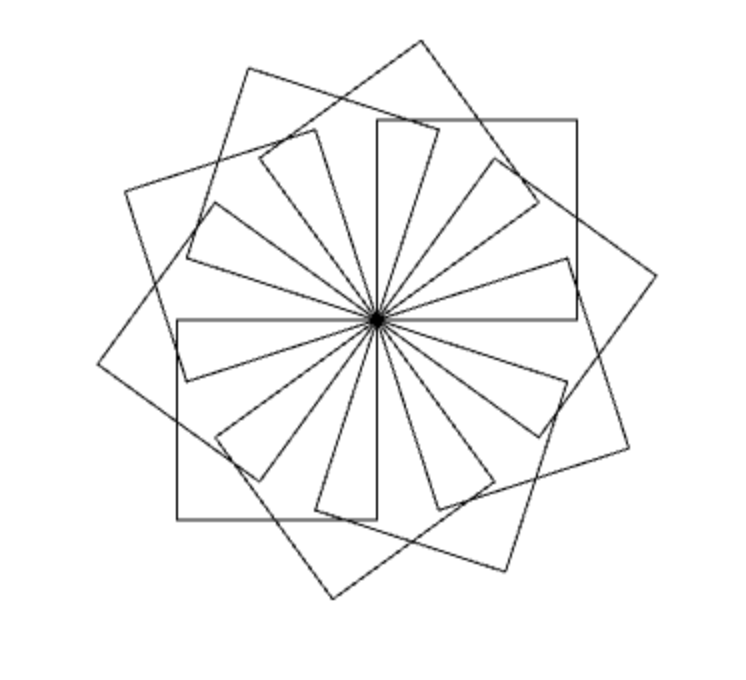
\includegraphics[width=0.2\pagewidth]{Grundlagen_Info/00_Programmieren/Figures/viereck_blume}
\end{figure}
\begin{myanswer}
	\lstinputlisting[language=Python,caption=\texttt{blume.py},label=listing:blume]{Grundlagen_Info/00_Programmieren/Skript/Code/K02_Intro/blume.py}
\end{myanswer}
\end{myexercise}

\begin{myexercise}\label{myexercise:Flaggen}
	\begin{enumerate}
		\item Zeichnen Sie die quadratische Schweizer Flagge \emoji{switzerland} (\textbf{Tipp}: zuerst ohne Farben, danach farbig). Um eine Form auszufüllen, schauen Sie sich die Funktionen \lstinline|t.fillcolor()|, \lstinline|t.begin_fill()| und \lstinline|t.end_fill()| in der \href{https://docs.python.org/3/library/turtle.html}{turtle-Dokumentation} an. Suchen Sie nach dem Begriff \texttt{\enquote{fill}} mit dem Shortcut \keys{\ctrl+F} (Windows) oder \keys{\cmd+F} (MacOS).
		\item Zeichnen Sie die Flagge des Kantons Zürich (quadratisch):
		      \begin{center}
			      
\includegraphics[width=0.1\linewidth]{Grundlagen_Info/00_Programmieren/Figures/Flag_of_Canton_of_Zürich}
			      \definecolor{zhblue}{RGB}{0,112,180}\\
			      \textcolor{zhblue}{Farbe \enquote{Züri-Blau}}: \texttt{(0 / 255, 112 / 255, 180 / 255)}
		      \end{center}
		\item Zeichnen Sie eine horizontal dreigeteilte, rechteckige Flagge (wie etwa die Flagge Frankreichs \emoji{flag-france} oder Italiens \emoji{flag-italy}).
	\end{enumerate}
	\begin{myanswer}
		Diese Musterlösung finden Sie in \cref{sec:K02_sol}.
	\end{myanswer}
\end{myexercise}

\begin{mychallenge}
	In den folgenden beiden Aufgaben müssen Sie dasselbe tun wie in Teil 3 von \cref{myexercise:Flaggen} aber mit den folgenden Ergänzungen:
	\begin{enumerate}
		\item Die Breite jedes einzelnen der drei Rechtecke soll vom Programm bei jeder Ausführung individuell zufällig gewählt werden (das Programm soll zufällig drei Werte wählen).
		\item Nun sollen zusätzlich zu den Breiten auch noch die Farben jeder der drei Rechtecksflächen zufällig gewählt werden.
	\end{enumerate}
\end{mychallenge}

\clearpage
\begin{myoverview}[\texttt{turtle}-Befehle]
	\leavevmode
	\begin{table}[H]
		\centering
		\begin{tabular}{lll}
			\midrule
			\textbf{Kurzform}            & \textbf{Langform}            & \textbf{Beschreibung}                                                                                   \\
			\midrule
			\lstinline|t.fd(x)|          & \lstinline|t.forward(x)|     & bewegt die Turtle um \lstinline|x| Schritte vorwärts                                                    \\
			\lstinline|t.bk(x)|          & \lstinline|t.backward(x)|    & bewegt die Turtle um \lstinline|x| Schritte rückwärts                                                   \\
			\lstinline|t.rt(x)|          & \lstinline|t.right(x)|       & dreht die Turtle um \lstinline|x| Grad nach rechts                                                      \\
			\lstinline|t.lt(x)|          & \lstinline|t.left(x)|        & dreht die Turtle um \lstinline|x| Grad nach links                                                       \\
			\lstinline|t.color(c)|       & \lstinline|t.color(c)|       & setzt die Zeichenfarbe auf \lstinline|c| (z.\,B.\ \lstinline|"red"|)                                    \\
			\lstinline|t.begin_fill()|   & \lstinline|t.begin_fill()|   & Start des Füllbereichs                                                                                  \\
			\lstinline|t.end_fill()|     & \lstinline|t.end_fill()|     & Ende des Füllbereichs (füllt Fläche)                                                                    \\
			\lstinline|t.pu()|           & \lstinline|t.penup()|        & hebt den Stift (es wird nicht mehr gezeichnet)                                                          \\
			\lstinline|t.pd()|           & \lstinline|t.pendown()|      & senkt den Stift (es wird wieder gezeichnet)                                                             \\
			\lstinline|t.ht()|           & \lstinline|t.hideturtle()|   & versteckt die Turtle                                                                                    \\
			\lstinline|t.st()|           & \lstinline|t.showturtle()|   & zeigt die Turtle                                                                                        \\
			\lstinline|t.speed(x)|       & \lstinline|t.speed(x)|       & Geschwindigkeit setzen (\lstinline|0| = schnellste)                                                     \\
			\lstinline|t.goto(x, y)|     & \lstinline|t.goto(x, y)|     & bewegt die Turtle zu den Koordinaten \lstinline|(x, y)|                                                 \\
			\lstinline|t.circle(r)|      & \lstinline|t.circle(r)|      & zeichnet einen Kreis mit Radius \lstinline|r|                                                           \\
			\lstinline|t.tracer(False)|  & \lstinline|t.tracer(False)|  & zeigt direkt das Resultat (ohne Animation)\footnote{Funktioniert nicht in allen Programmier-Umgebungen} \\
			\lstinline|t.teleport(x, y)| & \lstinline|t.teleport(x, y)| & teleportiert die Turtle zu \lstinline|(x, y)|                                                           \\
			\midrule
		\end{tabular}
		\caption{Zusammenfassung nützlicher \texttt{turtle}-Befehle}
	\end{table}
\end{myoverview}

\iftoggle{exerciseonly}{}{%
	\clearpage

	\section{Längere Lösungen}\label{sec:K02_sol}

	\begin{myanswer}[myexercise:dreizack]
		\lstinputlisting[language=Python,caption=\texttt{dreizack.py},label=listing:dreizack]{Grundlagen_Info/00_Programmieren/Skript/Code/K02_Intro/dreizack.py}
	\end{myanswer}
	%
	\begin{myanswer}[myexercise:Flaggen]
		\begin{enumerate}
			\item\leavevmode
			      \lstinputlisting[language=Python,caption=\texttt{schweizer\_kreuz.py},label=listing:schweizer]{Grundlagen_Info/00_Programmieren/Skript/Code/K02_Intro/schweizer_kreuz.py}
			\item\leavevmode
			      \lstinputlisting[language=Python,caption=\texttt{zueri\_flagge.py},label=listing:zhflagge]{Grundlagen_Info/00_Programmieren/Skript/Code/K02_Intro/zueri_flagge.py}
			\item\leavevmode
			      \lstinputlisting[language=Python,caption=\texttt{flagge\_dreiteil.py},label=listing:flaggedreiteil]{Grundlagen_Info/00_Programmieren/Skript/Code/K02_Intro/flagge_dreiteil.py}
		\end{enumerate}
	\end{myanswer}
}
